\documentclass[11pt]{report}
\pagestyle{myheadings}
\markright{Group 13\hfill FLAMeS \hfill}
\usepackage{pdflscape}
\usepackage{longtable}
\usepackage{multirow}
\usepackage{enumerate}
\usepackage[printonlyused]{acronym}
\usepackage{multirow}
\usepackage{graphicx}
\usepackage{wrapfig}
\usepackage{subfig}
\usepackage{amsmath}
\usepackage{url}
\usepackage{fixltx2e}
\usepackage{booktabs}
\usepackage{rotating}
\usepackage{bbding}
\usepackage{fancyhdr}

\topmargin -1.5cm
\oddsidemargin -0.04cm 
\evensidemargin -0.04cm 
\textwidth 16.59cm 
\textheight 21.94cm 
\parskip 7.2pt 

\setcounter{secnumdepth}{5}
\setcounter{tocdepth}{2}
\pagenumbering{roman}

\pagestyle{fancy}

\renewcommand{\headrulewidth}{0 pt}
\begin{document}
\chapter{Stuff}



\label{RiskMan}
The main objective of the technical risk assessment is to determine the reliability compared to the possible (functional or financial) consequences per specific event. To be able to determine any of these reliabilities, a definition of reliability should be stated. In this case, reliability is formulated as:
\begin{quote}
\emph{The probability that a specific (part of a) subsystem will function without endangering the top level requirements over the expected lifetime.}
\end{quote}


Next to formulating the definition of reliability, it should be noted that the determined reliabilities in this section are relative reliabilities, i.e. the probability that a particular subsystem outperforms another subsystem with the same core function in terms of reliability. Hence, no absolute values of reliability are determined in this section. The relative reliabilities allow for comparison material during the trade-off between multiple design options. 
The risk assessment analysis is divided into four main sections: 
\begin{enumerate}[I]
	\item Ground segment (before vehicle leaves Earth's atmosphere)
	\item During mission
	\item Measurement protocol
	\item Post-mission
\end{enumerate}
The possible events, with their respective reliability, are outlined in these sections and after that the expected consequences are shortly explained. 

\section{Ground Segment}
\label{blTRAGs}
\begin{enumerate}[A]
	\item  \textbf{\textit{Financial}} \\\\
\textit{A1. Insufficient funds or low market-demand}\\
The approximate costs are determined in the cost budget. The mission data and the final results can be very interesting for a vast number of commercial parties and research or educational facilities. Every space mission is created for at least one specific (user-demanded) requirement set by a user. This third party is responsible for covering the cost. Since the space mission is developed after this request is set, the probability that there will be insufficient funds is low (especially when more than one company can be considered as the user). However, the consequence can be severe if the funds are not enough to start or continue the development. 

	\item  \textbf{\textit{Technological readiness}} \\\\
\textit{B1. Technology for level zero requirements are not available}\\
If the technology for measuring, detecting or processing the level zero requirements is 	not available at present, the requirements cannot be met and alternatives should be devised, or the mission should be terminated. In our case, the technical readiness level of the 	payload is relatively high and hence has a high reliability. If, however, the specific 	payload would have a low technical readiness level, the mission should be terminated or 	delayed. Therefore, it has important consequences to the mission.

	\item  \textbf{\textit{Launch}} \\\\
\textit{C1. Total launch failure}\\
Total failure indicates complete failure of the launch vehicle and all laser swarm 	constellation components. Needless to say, the probability of occurrence is relatively low; however, the consequences of this event are catastrophic.

\textit{C2. Partial launch failure}\\
Partial launch failure indicates non-complete failure of laser swarm constellation components, i.e. some of the satellites (more receivers and one emitter) can still perform core tasks. Considering historical launch data, the probability that a partial failure will occur during launch is relatively low. The consequence can be very different, depending on which part (or what fraction) of the constellation cannot perform its core task. If one of the receivers will be destroyed, the level zero requirements might still be achievable. However, if the emitter is (partially) destroyed, the mission will surely be endangered. 

\textit{C3. Delayed vehicle launch}\\
Delaying the vehicle launch is not particularly a problem from the technological side of the mission; however, it will affect the financial situation. Next to the fact that the data and results are delayed, extra costs will be imposed due to an increase in launch vehicle pad costs, extra personnel costs and others. The probability of this event is actually not that low, since it is dependent on a lot of criteria like third-party companies, the weather, and atmospheric properties. The consequences are mainly financial.

\section{During Mission}
\label{blTRADm}
	\item  \textbf{\textit{Orbit accuracy }} \\\\
\textit{D1. One or more satellites are in a wrong orbit.}\\
After launch and orbit initializing, it is possible one or more of the satellites are in a wrong orbit. If this deviation from the desired orbit is relatively small, the ADCS subsystem should be able to cope with this minor error and adjust the orbit. If the altitude error is large, major altitude changes should be imposed. Assuming a low to moderate error, the consequence is not really severe if the ADCS system is working properly. The chance of actually putting a satellite in the wrong orbit is also relatively small.

In the next section, the reliability of the ADCS subsystems is compared. The reliability of the systems is considered independently, but the consequences of failure are equal for all subsystems and thus shall not be inspected individually. The consequences are severe considering not only the loss of pointing accuracy, but also a decrease in vehicle stability and the total failure of altitude control.  	

	\item  \textbf{\textit{Active systems}} \\\\
\textit{E1. Actuators}\\

\textit{E1a. Thrusters (hot and cold gas) for orbit maintenance.}\\ 
The thruster systems are used for advanced orbit keeping. The system is dependent on fuel consumption, combustion and mechanical properties. Each of these dependencies decreases the reliability. 

\textit{E1b. Reaction wheels.}\\ 
Mechanical reliability is an import aspect for using active reaction wheels. 

\textit{E1c. Magnetic torquers}\\ 
The magnetic torquers interact with the Earth's magnetic field, creating compensating torques to induce stability. Reliability is high due to the fact that the magnetic field is known and the system is dependent on a low number of parameters.

\textit{E2. Sensors}\\ 
Assuming a high technical readiness level of the sensors, the reliability is considered high. Also, the consequences of failure are high as the continuation of the mission may be impaired.

	\item  \textbf{\textit{Positioning system}} \\\\
\textit{F1. GPS receiver failure}\\
The probability of failure for the GPS system is on the low side assuming the equipment is properly shielded. However if it should fail the mission is most likely lost, as is the satellite.

	\item  \textbf{\textit{Electric Power System (EPS)}} \\\\
\textit{G1. Solar Panels}\\

\textit{G1a. Solar panel deflection error or mechanical failure.}\\ 
During launch, the solar panels are retracted to achieve the lowest volume possible. During the initializing of the mission (assuming the spacecraft is in the right orbit), the solar panels need to be deployed. Errors can occur due to mechanical reasons or external disturbances. The probability of this is on the low side. The consequence can be however that the effective solar panel area is decreased and hence a decrease in available electrical power will occur. This makes the consequences rather large. Any other mechanical failure (broken joints, internal PN-junction failure, or a loss of an entire solar panel) will have severe consequences as well. 

\textit{G1b. Solar panel characteristics reliability (degradation).}\\ Degradation of solar panels should always be considered during mission development. Since this is (or should be) known upfront, the consequences are relatively small. The probability of this actually happening is nearly 100\%.

\textit{G1c. Severe degradation (due to external phenomenon)}\\ 
Atomic oxygen, hazardous radiation, debris collision and other external factors can influence the performance of the solar panels. Since these are not known from the start, it is difficult to cope with them. The probability of this happening is small, but will have severe consequences.\\\\

\textit{G2. Batteries}\\

\textit{G2a. Initial internal failure}\\ 
Considering a high level of technical readiness, the internal reliability is high. The consequences do alter the functional capacity of the mission, since no energy can be stored if the energy capacity system would completely fail, meaning that during eclipse no energy usage can occur. 

\textit{G2b. Decrease in capacity}\\ 
Considering a high level of technical readiness, the reliability is high. Consequences are low, because they are known and should be part of the mission analysis.

\section{Measurement Protocol}
\label{blTRAMp}
Since actual measurements are an important level zero requirement, the consequence of the items in the measurement protocol are all catastrophic. Unless stated otherwise, the consequences in the following section can thus be stated in this way.

\begin{description}
\item[\textit{Measurement}]
\end{description}
	\item\textbf{\textit{Emitter}} \\\\
\textit{H1. Laser pulses cannot be sent or no photon are generated}\\ With a high level of technical readiness, the reliability is high.

\textit{H2. Pointing towards nadir}\\
This is dependent on ADCS risks.

\textit{H3. Laser notifies receiver (time adjustment)}\\ 
With a high level of technical readiness, the reliability is high.

\textit{H4. Laser degradation}\\
Laser degradation is dependent on multiple parameters: thermal properties, input power interval, external factors and internal mechanical errors (manufacturing or design errors). However, due to extensive research and development concerning laser technology, the probability of severe laser degradation within the lifetime is relatively low. 

	\item\textbf{\textit{Receiver}} \\\\
\textit{I1. Pointing towards the target} \\
This is dependent on ADCS risks.

\textit{I2. Receive and detect photons}\\ 
The \ac{SPAD} is used to detect incoming photons, the actual technology is space qualified and as such the probability of missing photons is minimal. Furthermore the optical construction used in conjunction with the \acs{SMAD} leaves a minimal probability of missing photons. 

\textit{I3. Turn photon into electrical signal}\\ 
With the high level of technical readiness, the reliability is high as well.

\begin{description}
\item[\textit{Communication}]
\end{description}
	\item\textbf{\textit{Inter satellite communication}} \\\\
\textit{J1. Determine relative position receiver and emitter}\\ 
Due to the high technical readiness, the reliability is high.

\textit{J2. Time differences}\\ 
Due to the high technical readiness, the reliability is high.

	\item\textbf{\textit{Data handling}} \\\\
\textit{K1. Store data/ make data package}\\ 
With a high level of technical readiness, the reliability is high.

\textit{K2. Transmit package}\\ 
With a high level of technical readiness and relative low-tech technology, the reliability is high.

\textit{K3. Interpreted results}\\ 
Historical data comparisons for the interpretation of altimetry missions are sufficient, but not elaborate. However, the reliability is still on the high side.

\textit{K4. Reproduce terrain model}\\
Historical data comparisons for the interpretation of altimetry missions are sufficient, but not elaborate. However, the reliability is still relatively high.
 
	\item\textbf{\textit{Housekeeping/ Ground communication}} \\\\
\textit{L1. Housekeeping data from ground station to satellite}\\ 
Considering a high level of technical readiness level, the reliability is high.

\textit{L2. Adjusting space segment characteristics}\\ 
Considering a high level of technical readiness level, the reliability is high.

	\item\textbf{\textit{Structural}} \\\\
\textit{M1. Joints}\\ 
Considering a high level of technical readiness, the reliability is high.

\textit{M2. Connection points}\\ 
Considering a high level of technical readiness, the reliability is high.

\textit{M3. Thermal limits of the laser emitter}\\ 
Thermal limits will alter the characteristics of pretty much all subsystems. Using the system discussed on page \pageref{opticalthermal} the reliability is high, but a failure of this system would mean the laser overheats rapidly. Thus seriously endangering the mission.

\textit{M4. Fatigue}\\ 
High-cycle loading is usually not present (except for momentum wheels) and should therefore only play a minor role. The probability is low. The consequences are medium to high if high-cycle loading will lead to fatigue and hence partial failure.

\textit{M5. Electrical overlay failure}\\ 
This event is dependent on the reliability of the EPS.

\textit{M6. Launch loads} \\
Due to large forces and vibrations during launch, the structure of the satellite can fail. Since the launch loads are well known the reliability is low, the consequences can be severe.

	\item\textbf{\textit{External}} \\\\
\textit{N1. Debris collision}\\ 
Unknown external phenomenon. The probability of this event causing total failure, which is a function of multiple parameters like orbit and celestial position, is low to medium. 

\textit{N2. Dangerous radiation}\\ 
Unknown external phenomenon. The probability of this event causing total failure, which is a function of multiple parameters like orbit and celestial position, is low to medium. 

\textit{N3. Charged particles collision}\\ 
Unknown external phenomenon. The probability of this event causing total failure, which is a function of multiple parameters like orbit and celestial position, is low to medium. 

\textit{N5. Politics or international influence}\\ 
Political decisions or international influences can alter the space mission considerably.  With altimetry missions, the probability of these external influences causing a delayed or complete stop of the mission is negligible. The consequences, however, could be very severe. 

\textit{N6. Classified information (military)}\\ 
Some parts of the measurement are considered classified information, for example military ground stations or governmental classified areas. The government and/ or military can pressure the vehicle engineers to keep certain information classified. However, if this is the case, most of the measurements still can be taken and analyzed. So while the probability is medium, the consequences are very low.

\section{Post-Mission}
\label{blTRAPm}
	\item\textbf{\textit{Satellite decommission}} \\\\
\textit{O1. Decommission LEO}\\ 
At the end of life the satellites have to be decommissioned to allow new missions to take their place. To decommission satellites in \ac{LEO} one could just wait a couple of years and air drag will cause the satellites orbit to degrade to the point when they can burn up in the atmosphere, so the consequences are low. However, it is desirable to have the satellites burn up faster, so as to remove the risks of satellite collision. The probability to no longer be able to eject the satellite from orbit depends on whether or not its propulsion system is still working; as such this probability is low.

\section{Risk Control}
\label{blTRARC}
Sometimes it is possible to decrease the failure probability. For example, A1, E1a and H4 could be the top 3 risk segment. Failure probability of A1 can be pulled down by doing detailed market analysis. In case of F1a, safe combustion performance as well as fuel consumption can be tested and modified in a laboratory environment to increase the thrusters' reliability. Laser degradation (H4) is crucial in the system, and reliable energy source should be used to prevent failure. Meanwhile, thermal control can be performed to achieve high reliability of the laser emitter.  

\begin{figure} [h]
	\begin{center}
 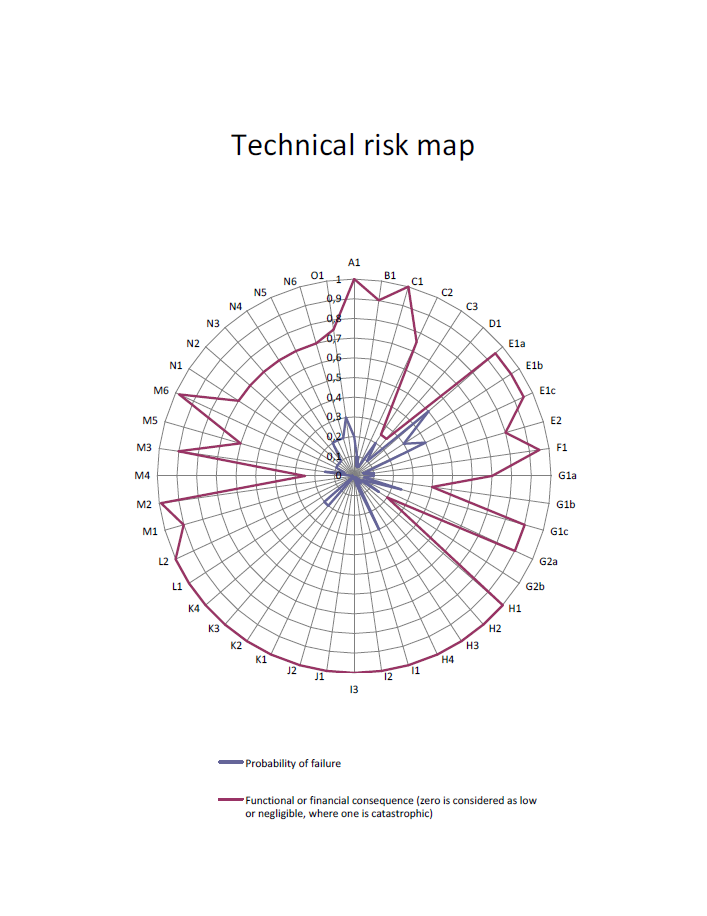
\includegraphics[trim = 0mm 0mm 0mm 35mm, clip,width=1.0\textwidth,angle=0]{img/TRA_RM.png}	
	\caption{Technical Risk Map}
	\label{TRA_RM}
	\end{center}
\end{figure}

\end{enumerate}






\end{document}